\documentclass[border=3pt]{standalone}
\usepackage{tikz}
\usetikzlibrary{arrows.meta,calc,positioning}
\tikzset{st/.style={draw, thick, rounded corners=3pt, minimum width=20mm, minimum height=11mm, font=\sffamily\small, align=center},
  pin/.style={-{Stealth[length=5pt]}, thick}}
\begin{document}
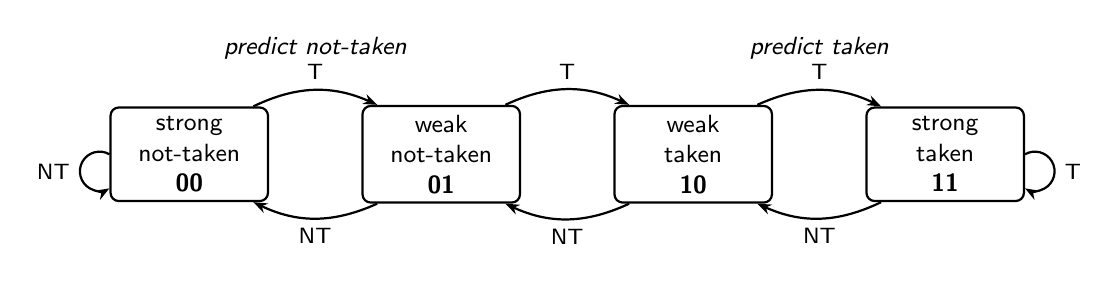
\begin{tikzpicture}[font=\sffamily\footnotesize]
  \node[st] (sn) at (0,0)    {strong\\not-taken\\\textbf{00}};
  \node[st] (wn) at (3.2,0)  {weak\\not-taken\\\textbf{01}};
  \node[st] (wt) at (6.4,0)  {weak\\taken\\\textbf{10}};
  \node[st] (st) at (9.6,0)  {strong\\taken\\\textbf{11}};
  % taken edges (above, left to right)
  \draw[pin] ($(sn.north east)+(-2mm,0)$) to[bend left=25] node[above]{T} ($(wn.north west)+(2mm,0)$);
  \draw[pin] ($(wn.north east)+(-2mm,0)$) to[bend left=25] node[above]{T} ($(wt.north west)+(2mm,0)$);
  \draw[pin] ($(wt.north east)+(-2mm,0)$) to[bend left=25] node[above]{T} ($(st.north west)+(2mm,0)$);
  % not-taken edges (below, right to left)
  \draw[pin] ($(st.south west)+(2mm,0)$) to[bend left=25] node[below]{NT} ($(wt.south east)+(-2mm,0)$);
  \draw[pin] ($(wt.south west)+(2mm,0)$) to[bend left=25] node[below]{NT} ($(wn.south east)+(-2mm,0)$);
  \draw[pin] ($(wn.south west)+(2mm,0)$) to[bend left=25] node[below]{NT} ($(sn.south east)+(-2mm,0)$);
  % self loops
  \draw[pin] (sn.west) arc (60:300:2.5mm) node[pos=0.5, left]{NT} ;
  \draw[pin] (st.east) arc (120:-120:2.5mm) node[pos=0.5, right]{T};
  % prediction brackets
  \node[font=\sffamily\small\itshape] at (1.6,1.35) {predict not-taken};
  \node[font=\sffamily\small\itshape] at (8.0,1.35) {predict taken};
\end{tikzpicture}
\end{document}
